\chapter{Experiments}
\label{chap:4}
%

- parallel runs on the cluster

\section{Implementation}

\subsection{Problem environment}
In early test runs we used \texttt{Matlab} implementations of cart pole, acrobot, and mountain car adapted from \cite{joseCode}. But later we implemented OpenAI Gym to have a wide range of problem environments available and to have consistent rewarding functions. Otherwise, the rewarding function would depend on the source and therefore produce less comparable results.



\subsection{Gaussian Process Regression}

(difference between full covariance and cov vector)

Instead of calculating the inverse of $K_n$ in \eqref{eq:meanGauss} we use the lower Cholesky decomposed matrix:

$$LL^\top=K_n$$

This is considered faster and numerically more stable \cite{rasmussen2006gaussian}. The mean vector $\mu$ is then computed as follows:

\begin{equation} \label{eq:regression}
    \mu = K_n^{-1}\,y = (L\,L^{T})^{-1}\,y = (L^{-T}\,L^{-1})\,y = L^{-T}\,(L^{-1}\,y) = L^{T}\setminus(L \setminus y).
\end{equation}

The backslash operator denotes the matrix left division, so the solution $x=A\setminus b$ satisfies the system of linear equations $A\,x=b$.
Matrix $K_n$ must be positive definite for the cholesky decomposition. So we double the noise variance hyperparameter $\sigma_n^2$ from \eqref{eq:kNoise} until positive definiteness is achieved.

For the expected improvement function we only need the vector of variances. Instead of calculating the whole covariance matrix $V$ we can take a shortcut. All elements on the diagonal of $K(X_*,X_*)$ equal $\sigma_f$ because the difference between one $x_*$ and the same $x_*$ is zero. Therefore we write:

$$L_k = L \setminus K(X_*,X)$$

$$v = \sigma_f - \sum_{\text{rows}} (L_k \circ L_k).$$

This adaptation is inspired by \cite{nandoCode} and reduces the computational effort drastically.

For the whole covariance matrix we also avoid calculating the matrix inverse:

$$V = K(X_*,X_*) - (L_k^\top L_k)^\top $$

\subsection{Hyper Parameter Optimization}
Especially for the trajectory kernel we want a hyper parameter optimization, because all the values of the distance matrix $D$ may get very big. When dividing by a well tuned hyper parameter $sigma_l$ before applying the exponential function \eqref{eq:trajKernel}, we avoid getting a zero kernel matrix $K$.\\

When calculating $\log(|K_n|)$ for the hyperparameter optimization \eqref{eq:hypOpt}, again we use the Cholesky decomposition of $K$. Thus the determinant transforms to
$$|K_n|=|L\,L^{T}|=|L|\,|L^{T}|=|L|\,|L|=|L|^{2}.$$

Since the determinant of the Cholesky decomposed matrix,
$$|L| = \textstyle\prod_{i} L_{ii},$$
is the product of its diagonal elements, we can transform this into a numerically more stable version:

$$\log(|K_n|) = \log(|L|^{2}) = 2\,\log(|L|) = 2\,\log(\textstyle\prod_{i} L_{ii}) = 2\textstyle\sum_{i} \log(L_{ii}).$$

The computation of $K_y^{-1}y$ in \eqref{eq:hypOpt} is done by the same method we already use in the Gaussian process \eqref{eq:regression}.

\subsection{Estimation of Trajectory Kernel Function Values}

We estimate the divergence values, because the computational effort will be greatly reduced\cite{wilson2014using}. We use a Monte-Carlo estimate for the approximation

$$\hat{D}(x_{ i }, x_{ j }) = \sum _{\xi \in \xi_i} \log\left( \frac{P(\xi|x_{ i })}{P(\xi|x_{ j })} \right) + \sum _{\xi \in \xi_j} \log\left( \frac{P(\xi|x_{ j })}{P(\xi|x_{ i })} \right) $$

of the divergences between policies with already sampled trajectories. Here $\xi_i$ is the set of trajectories generated by policy $x_i$. For our gaussian process regression we also need a distance measure between a policy with known trajectories and new policies with unknown trajectories. Since there is no closed form solution to this we use the importance sampled divergence

$$\hat{D}(x_{ new }, x_{ j }) = \sum _{\xi \in \xi_j} \left[\frac{P(\xi|x_{ new })}{P(\xi|x_{ j })}\,\log\left(\frac{P(\xi|x_{new})}{P(\xi|x_{j})}\right)+\log\left(\frac{P(\xi|x_{ j })}{P(\xi|x_{ new })}\right)\right] $$

to estimate the divergence between the new policy $x_{new}$ and the policy $x_j$ with already sampled trajectories $\xi_j$.

Since we only have a ratio of transitioning probabilities present in our trajectory kernel we can reduce the logarithmic term to:

\begin{align*}
    \log\left(\frac{P(\xi|x_i)}{P(\xi|x_j)}\right)
    &= \log\left(\frac{P_{0}(s_{0}) \prod_{t=1}^{T} P_s(s_{t}|s_{t-1},a_{t-1}) P_{\pi}(a_{t-1}|s_{t-1},x_i)}{P_{0}(s_{0}) \prod_{t=1}^{T} P_s(s_{t}|s_{t-1},a_{t-1}) P_{\pi}(a_{t-1}|s_{t-1},x_j)}\right)\\
    &= \log\left(\prod_{t=1}^{T}\frac{ P_{\pi}(a_{t-1}|s_{t-1},x_i)}{P_{\pi}(a_{t-1}|s_{t-1},x_j)}\right)\\
    &= \sum_{t=1}^{T} \log \left(\frac{P_{\pi}(a_{t-1}|s_{t-1},x_i)}{P_{\pi}(a_{t-1}|s_{t-1},x_j)}\right).
\end{align*}


Summing up the logarithms in the end is also numerically more stable than taking the logarithm of the products.

\subsection{Action selection}

In continuous action space we use a linear policy to action mapping

$$a = f_s(s)^\top x + \epsilon_a,$$

with a small gaussian noise $\epsilon_a$ needed for stochastic policies. So the actions are Gaussian distributed:

$$a \sim \mathcal{N}(f_s(s) x,\epsilon_a^2).$$

In discrete action space environments we use a parametric soft-max action selection policy:

$$P(a|s)= \frac{\exp(f_s(s)^\top x_a)}{\sum_{i\in A} \exp(f_s(s)^\top x_i)}.$$

Again it consists of the linear mapping $f_s(s)^\top x$, and $A$ holds all possible actions. The resulting action is then sampled from the probability of action $a$ given state $s$.

The state feature function $f_s(s)$ is defined for each environment as shown below.

\section{Cart pole}


\begin{figure}
    \begin{center}
        \fbox{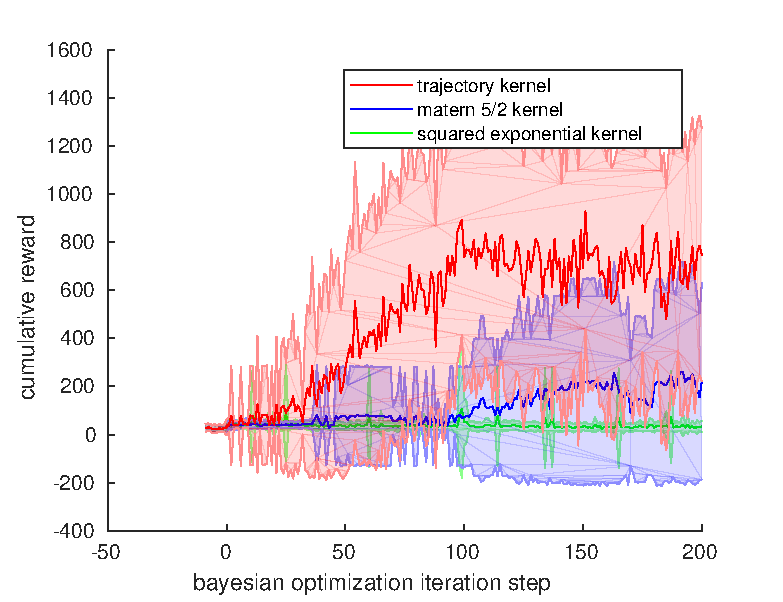
\includegraphics{/home/sebastian/Documents/bscThesis/img/cartpole_matlab_conti_oldreward.pdf}}
        \caption{Global opt, 4 dim. Mean and standard deviation from 32 trials of each kernel. Cartpole matlab implementation with old reward function, 1000 timesteps, and continuous action selection.}
    \end{center}
\end{figure}

\begin{figure}
    \begin{center}
        \fbox{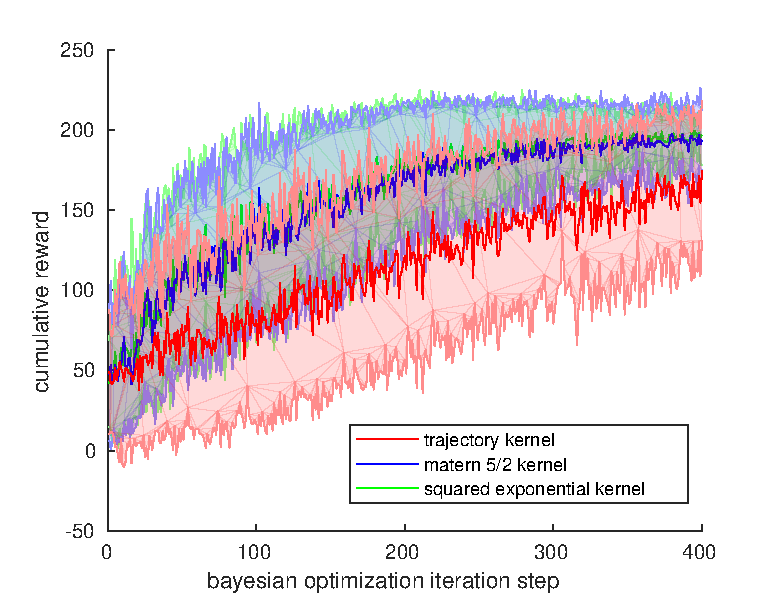
\includegraphics{/home/sebastian/Documents/bscThesis/img/cartpole_matlab_conti_newreward_local}}
        \caption{Local opt, 4 dim. Mean and standard deviation from 32 trials of each kernel. Cartpole matlab implementation with new reward function, 200 timesteps, and continuous action selection.}
    \end{center}
\end{figure}

\begin{figure}
    \begin{center}
        \fbox{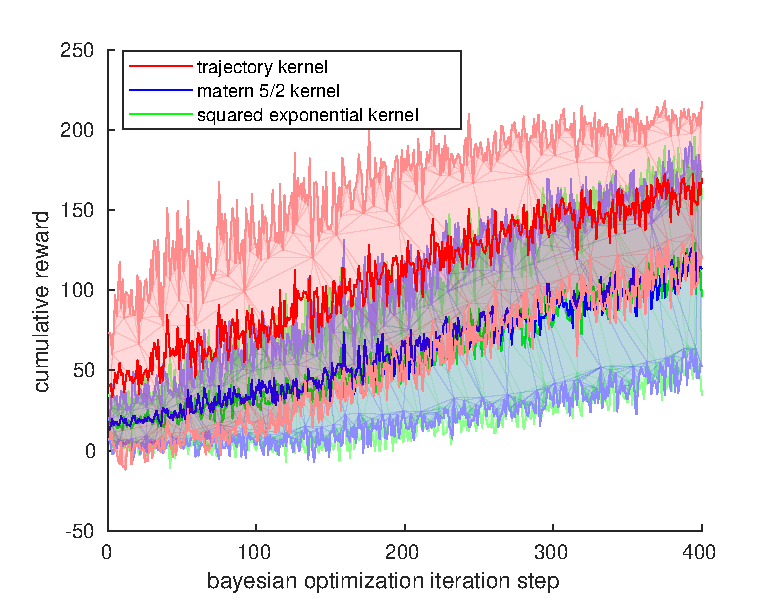
\includegraphics{/home/sebastian/Documents/bscThesis/img/cartpole_pygym_disc_local}}
        \caption{Local opt, 10 dim. Mean and standard deviation from 32 trials of each kernel. Cartpole python gym implementation, 200 timesteps, and discrete action selection.}
    \end{center}
\end{figure}
